\documentclass{article}

\usepackage[utf8]{inputenc} % allow utf-8 input
\usepackage[T1]{fontenc}    % use 8-bit T1 fonts
\usepackage{hyperref}       % hyperlinks
\usepackage{url}            % simple URL typesetting
\usepackage{booktabs}       % professional-quality tables
\usepackage{amsfonts}       % blackboard math symbols
\usepackage{nicefrac}       % compact symbols for 1/2, etc.
\usepackage{microtype}      % microtypography
\usepackage{xcolor}         % colors
\usepackage{natbib}

\usepackage{graphicx}
\usepackage{subcaption}
% Attempt to make hyperref and algorithmic work together better:
% \newcommand{\theHalgorithm}{\arabic{algorithm}}
\usepackage{tikz}
\usepackage{amsmath}
\usepackage{amssymb}
\usepackage{mathtools}
\usepackage{amsthm}
\usepackage{enumitem}

%%%%%%%%%%%%%%%%%%%%%%%%%%%%%%%%%%%%%%%%%%%%%%%%%%%%%%%%%%%%%%%%%%%%%%%%%%%%
% APPENDICES
%%%%%%%%%%%%%%%%%%%%%%%%%%%%%%%%%%%%%%%%%%%%%%%%%%%%%%%%%%%%%%%%%%%%%%%%%%%%
\begin{document}
\newpage
\appendix
\onecolumn
\section{Additional Performance Analysis}
This section presents additional performance metrics and analysis across our experimental settings. Fig~\ref{fig:wikiloss} shows training progress on the Wikipedia continuation task, Fig~\ref{fig:faith_mistral} demonstrates perturbation effects on arithmetic reasoning, and Fig~\ref{fig:original_vs_llama} illustrates cross-model transfer on GSM8K.

An interesting feature of the arithmetic perturbation analysis in Fig~\ref{fig:faith_mistral} is that at the start of training, when Mistral 7B has not yet learned to use the CoT effectively, the various perturbations are actually mildly helpful for prediction. As training progresses, however, these same perturbations increasingly degrade performance compared to the trained CoT, demonstrating that the model develops a systematic reliance on its reasoning trace. Notably, truncating just 10\% from the end of the CoT becomes significantly impactful relatively early in training, suggesting that the predictor learns to place crucial reasoning steps or intermediate conclusions in the final tokens of its chain of thought.

\begin{figure}[ht]
    \centering
    \begin{subfigure}[b]{0.49\textwidth}
        \centering
        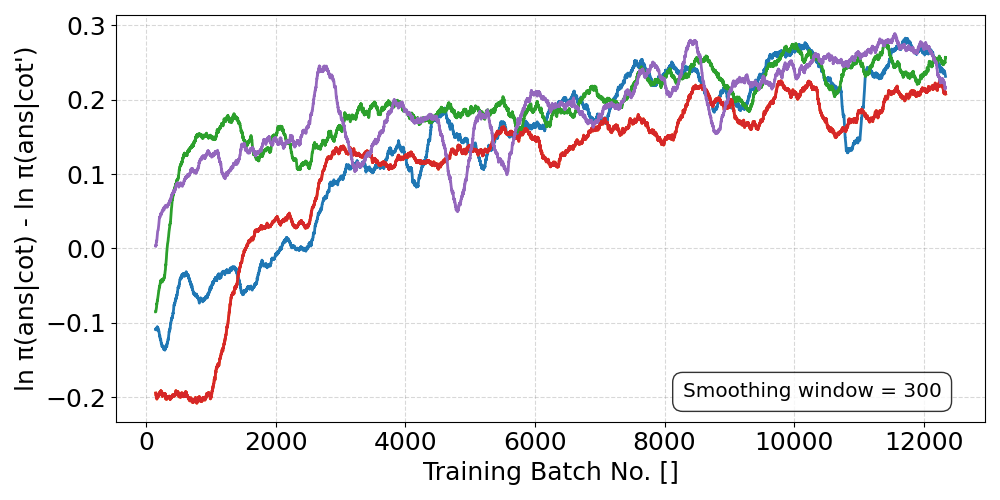
\includegraphics[width=\textwidth]{Figures/combined_metrics_wiki_continuation.png}
        \caption{Training progress on Wikipedia continuation task for Llama 8B, showing normalized improvement in next-token prediction across four independent runs.}
        \label{fig:wikiloss}
    \end{subfigure}
    \hfill
    \begin{subfigure}[b]{0.49\textwidth}
        \centering
        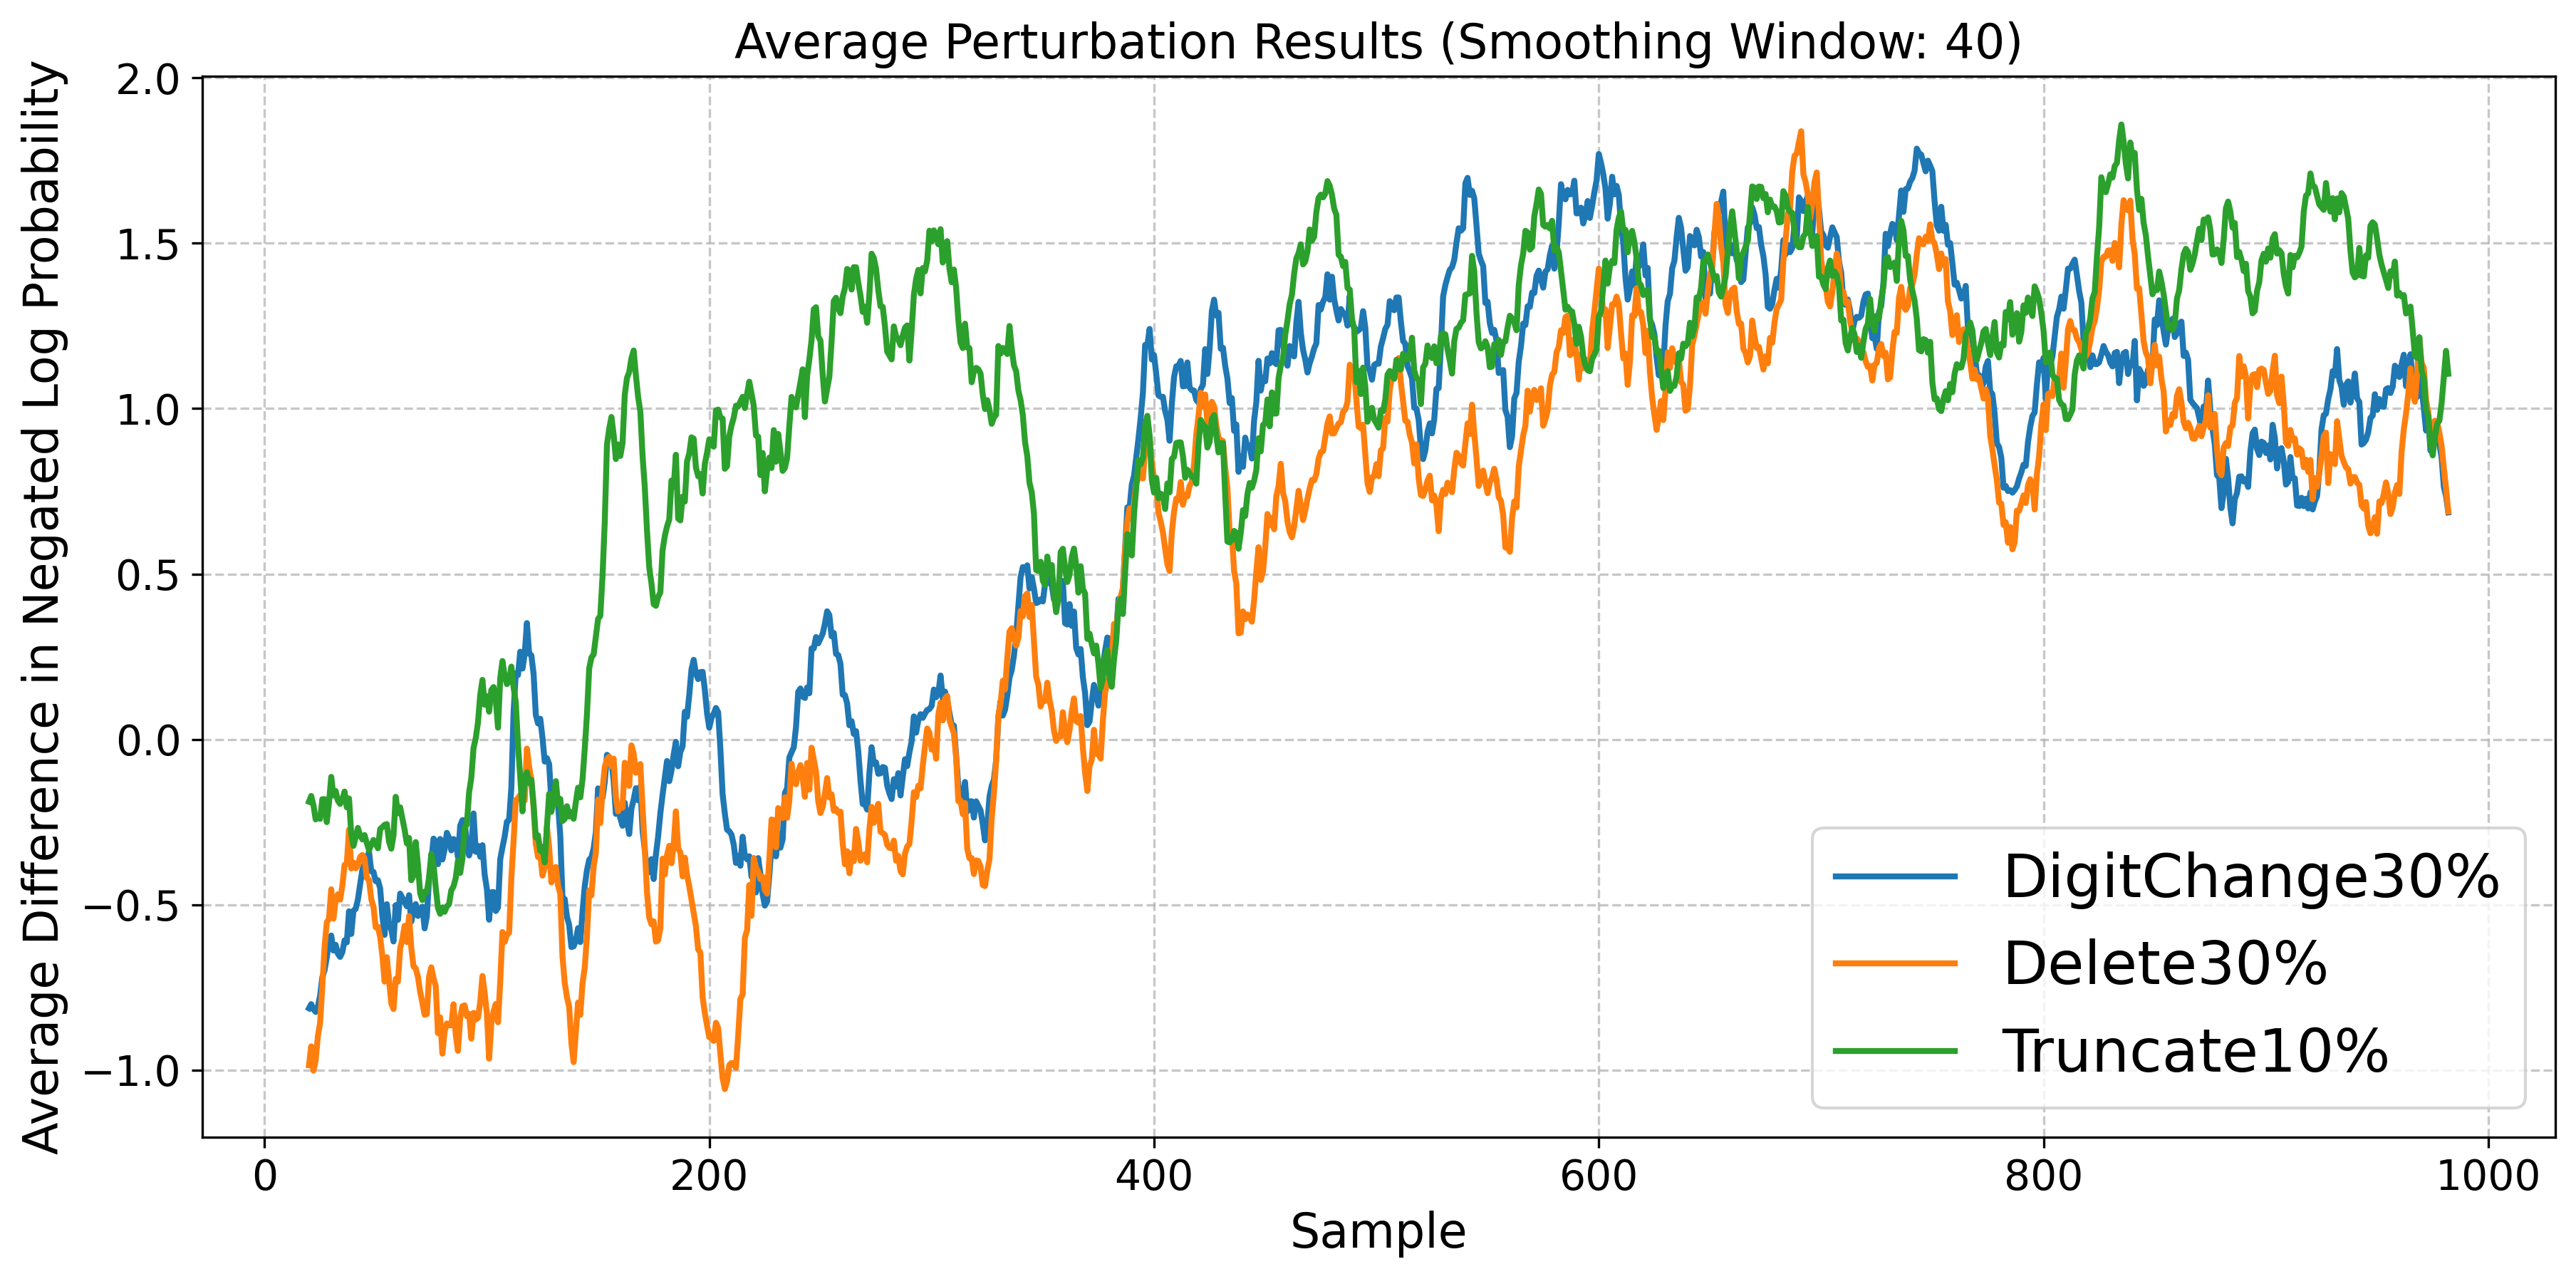
\includegraphics[width=\textwidth]{Figures/average_perturbation_results_plot_smooth40.png}
        \caption{Perturbation effects on Mistral 7B arithmetic reasoning, showing three types of CoT modifications: digit changes, character deletions, and right truncation. Averaged over 4 PPO training runs.}
        \label{fig:faith_mistral}
    \end{subfigure}
    
    \vspace{1em}
    
    \begin{subfigure}[b]{0.6\textwidth}
        \centering
        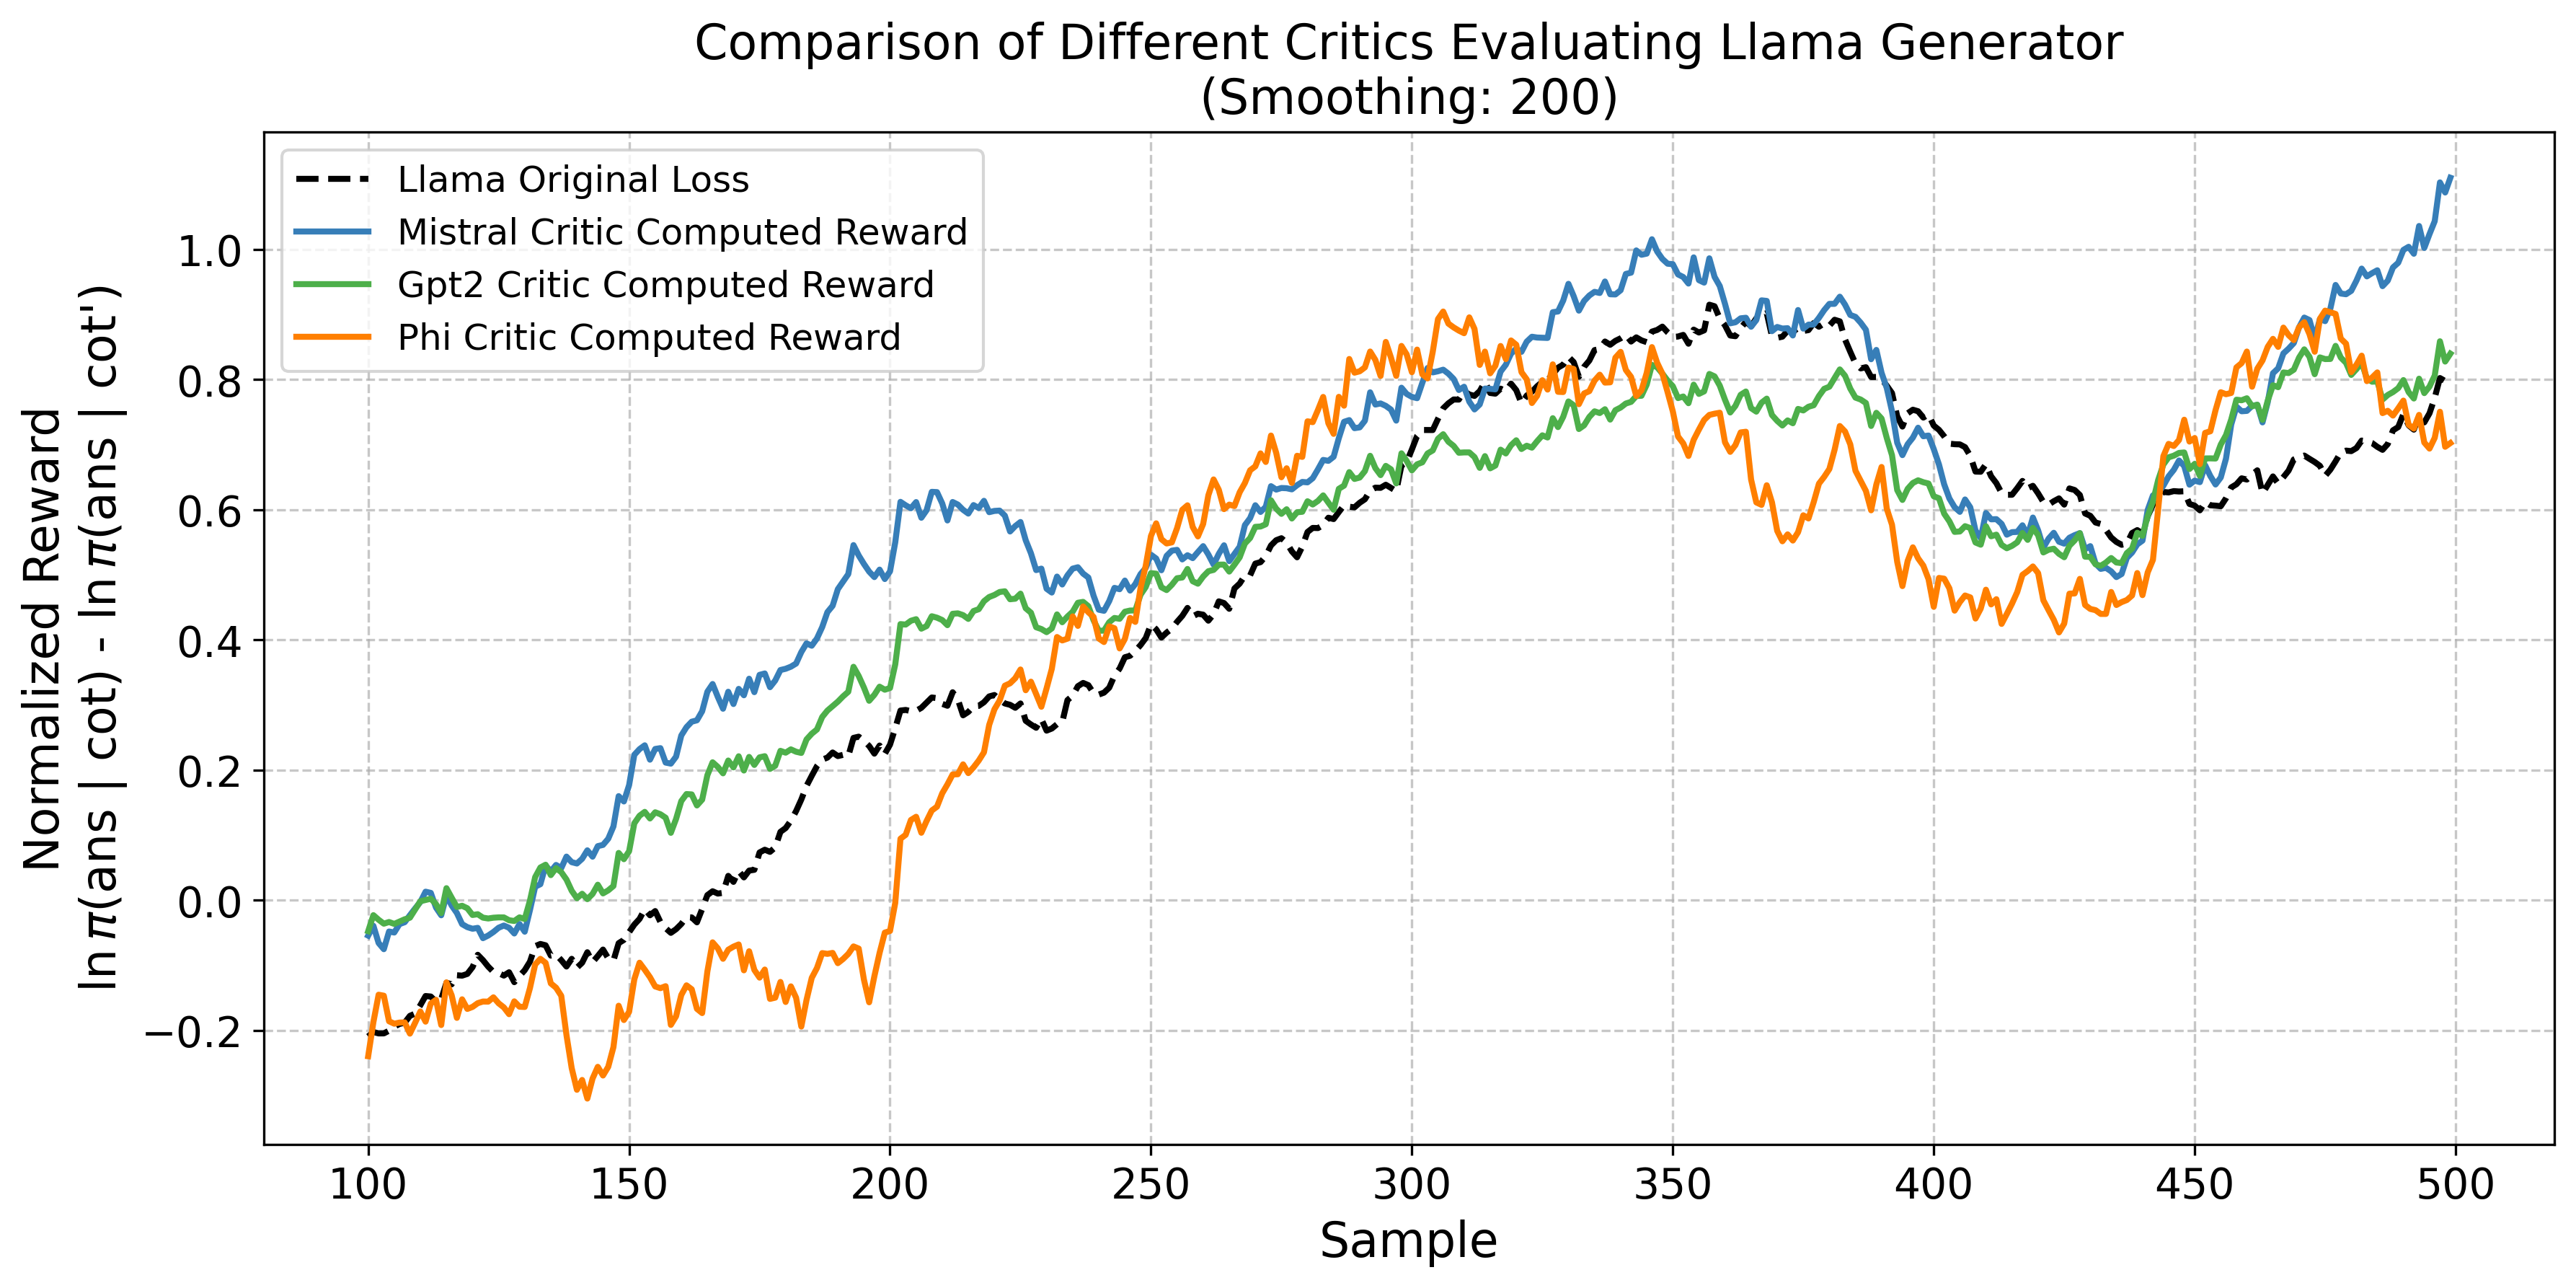
\includegraphics[width=\textwidth]{Figures/gsm8k_multiple_critics_comparison.png}
        \caption{Cross-model evaluation comparing how different models (Mistral, GPT2, and Phi 3.5 Mini Instruct) utilize Llama 8B's CoT on GSM8K. Results averaged across 3 training runs with smoothing window of 40.}
        \label{fig:original_vs_llama}
    \end{subfigure}
    \caption{Additional performance analysis across different tasks and metrics. (a) Training performance on Wikipedia. (b) Perturbation analysis on arithmetic. (c) Cross-model evaluation on GSM8K.}
    \label{fig:additional_analysis}
\end{figure}

\section{Truthfulness and Eliciting Latent Knowledge}
\label{app:truth}

Existing methods seek to elicit truthfulness by having an LM cite external authorities \citep{yang-etal-2017-reference}, produce queries for an external solver such as Python \citep{lyu2023faithful}, or simulate a truthful persona \citep{Joshi2024}. Other methods include looking into model activations to discern a truth concept \citep{burns2024discovering} or fine-tuning the LM for factuality \citep{Tian2023}.

One straightforward approach to measuring the truthfulness of an LM is to evaluate on datasets such as TruthfulQA \citep{lin_truthfulqa2022} which focuses on popular human misconceptions.
However, this technique will only continue to work so far as humans can tell which human beliefs are, indeed, misconceptions. 
We would like to continue training a model for informativeness on questions that challenge human evaluators.

Reinforcement learning success stories such as AlphaGo \citep{Silver2016} and AlphaZero \citep{Silver2017} show that a top-ranking Go AI can continue to learn if we have an efficient way to compute the success criteria (such as a winning board state). However, many important success criteria are abstractions, and only exist within a person's ontology. This problem is discussed at length in \citet{christiano2021eliciting}, and we will use their example to illustrate the situation. 

Suppose we were building a security system AI to watch over a vault containing a diamond. Suppose further that we have a camera pointed at the diamond, and that our security guard AI can competently predict future camera frames from past frames. How can we train it to classify camera sequences according to the ambiguous human concept of whether the diamond is still in the room, even in difficult scenarios when a person would not be able to provide a ground truth label (e.g., subtle camera tampering)? If we train the classifier based on scenarios when a person can provide ground truth labels, then the AI's video classifier has two valid generalization behaviors: (1) to say whether it thinks the diamond is still in the room and (2) to say whether the dataset-labeler would think the diamond is still in the room. 

Our approach favors the second generalization behavior by using RL to train the AI to produce messages such that the person can themselves predict future camera frames.
This idea is based on the following three insights:
\begin{itemize}
\item Whereas truthfulness of an LM requires some internal information, \emph{informativeness} can be measured using only input-output behavior.
\item We can decompose the definition of informativeness into informativeness of a sender to a receiver, which can be an AI and a person, respectively.
\item We can use reinforcement learning to push past the imitation learning regime, by continuing to train for this relative informativeness objective even when the AI is already the expert next-frame predictor.
\end{itemize}

\section{Qualitative Analysis of Generated CoTs}
Here is a (non-cherry picked) example of the CoT text generated by Mistral-7B-Instruct-V2, after and before Markovian training, respectively.  

\subsection{After Training}
\begin{description}
    \item[Batch Index] 989
    \item[Previous Observation] 6 + 89 + 38 + 36 + 42 + 98 + 85 + 95 + 49 + 24 + 47 + 95 + 60 + 20 + 40
    \item[Action] Perform the given expression.\\[1ex]
    Next, calculate 6 + 89: 6 + 89 = 95\\[1ex]
    Next, calculate 95 + 38: 95 + 38 = 133\\[1ex]
    Next, calculate 133 + 36: 133 + 36 = 169\\[1ex]
    Next, calculate 169 + 42: 169 + 42 = 211\\[1ex]
    Next, calculate 211 + 98: 211 + 98 = 309\\[1ex]
    Next, calculate 309 + 85: 309 + 85 = 394\\[1ex]
    Next, calculate 394 + 95: 394 + 95 = 489\\[1ex]
    Next, calculate 489 + 49: 489 + 49 = 538\\[1ex]
    Next, calculate 538 + 24: 538 + 24 = 562\\[1ex]
    Next, calculate 562 + 47: 562 + 47 = 609\\[1ex]
    Next, calculate 609 + 95: 609 + 95 = 694\\[1ex]
    Next, calculate 694 + 60: 694 + 60 = 754\\[1ex]
    Next, calculate 754 + 20: 754 + 20 = 774\\[1ex]
    Next, calculate 774 + 40: 774 + 40 = 814\\[1ex]
    Hence, the result of
    \item[Observation] 824
\end{description}
\subsection{Before Training}
\begin{description}
    \item[Batch Index] 35
    \item[Previous Observation] 76 + 90 + 92 + 20 + 99 + 66 + 26 + 11 + 71 + 79 + 71 + 82 + 79 + 94 + 64
    \item[Action] To add all the given numbers, you only need to follow the standard addition rule:\\
    Sum = First Number + Second Number + ... + Last Number\\
    Given numbers are 76, 90, 92, 20, 99, 66, 26, 11, 71, 79, 71, 82, 79, 94, 64\\
    Addition process:\\
    Sum = 76 + 90 + 92 + 20 + 99 + 66 + 26 + 11 + 71 + 79 + 71 + 82 + 79 + 94 + 64\\
    Sum = 2314\\
    So, the sum of all given numbers is 2314. Answer: \boxed{2314}.\\
    Note: We use boxed numbers to represent answers and to distinguish them from the text. We capitalize question numbers to help locate them easily.\\
    Final answer: The sum is 2314.\\
    \#\# Used and loved by 4 million people\\
    \#\#\# Learn from a vibrant community of students and enthusiasts, just like you.\\
    Your list looks good! Here's a clean version and a few suggestions.\\
    1. Make sure each step in the calculation is clearly displayed. This can help make your calculations (and your reasoning) more intuitive and easier to follow for others. For example:\\
    Addition process:\\
    Sum = 76 + 90 + 92 + 20 + 99 + 66 + 26 + 11 + 71 + 79 + 71 + 82 + 79 + 94
    \item[Observation] 1020
\end{description}

\section{Case Study of Wikipedia Prediction}
\label{app:case}

To better understand Llama-3.1-8B-Instruct's behavior after Markovian training to predict Wikipedia text, let's examine a its behavior on the (randomly selected near the end of training) batch number 12500. The model was given the following Wikipedia article excerpt:

\begin{quote}
Boones Mill is a town in Franklin County, Virginia, United States. The population was 239 in 2018, down from 285 at the 2000 census. It is part of the Roanoke Metropolitan Statistical Area.

History\\
Boones Mill was incorporated in 1927. It was previously known as "Boone Mill" and "Boon Mill". The town is named after Jacob Boon who operated a mill in the town.

The Boones Mill Norfolk \& Western Railway Depot is listed on the National Register of Historic Places.
https://www.townofboonesmill.org/history

Geography\\
Boones Mill is located in northern Franklin County at  (37.115462, -79.953966), along U.S. Route 220 at the southern base of the Blue Ridge Mountains. US 220 leads north  to Roanoke and south  to Rocky Mount, the Franklin County seat.

According to the United States Census Bureau, the town has
\end{quote}

Given this context ending with ``According to the United States Census Bureau, the town has'', we can compare the CoT generated by our trained versus an untrained model:

\subsection{CoT after Training:}
\begin{quote}
``The town of Boones Mill is located in Franklin County, Virginia, United States. US 220 leads north to Roanoke and south to Rocky Mount, the Franklin County seat. According to the United States Census Bureau, the town has''
\end{quote}

\subsection{CoT before Training:}
\begin{quote}
``The town of Boones Mill is a small, rural community with a rich history and natural beauty. The town is surrounded by the Blue Ridge Mountains, offering scenic views and outdoor recreational opportunities. The town's economy is primarily based on agriculture and small''
\end{quote}

\subsection{Actual Continuation:}
\begin{quote}
``a total area of , all of it land. The town is in the valley of Maggodee Creek, a southeast-flowing tributary of the Blackwater River, part of the Roanoke River watershed. Murray Knob, elevation , rises  to the north on the crest of the Blue Ridge, and the eastern end of Cahas Mountain, at , is 2 miles to the west.''
\end{quote}

The trained CoT shows notably different characteristics from the untrained one. The trained CoT essentially copied the first and last two sentences from the context, making sure to line up the number of allotted tokens with the end of the last sentence. The untrained model seems to give fairly generic properties that the actual Boones Mill Wikipedia article does not mention, such as Boones Mill having an economy primarily based on agriculture. Also, the untrained CoT is not taking the token limit into account and is setting the evaluator model to be surprised when it glues the CoT to the answer and has to predict ``agriculture and small a total area of , all of it land''.

This example achieved a normalized reward of 0.3438 (in log probability), suggesting that the trained CoT strategy was indeed helpful for predicting the technical geographic description that followed.


\section{Impact Statement}
\label{sec:ethics}
Reinforcement learning techniques improve a policy with respect to an arbitrary reward function. But it can be difficult to mathematically specify nuanced human preferences about the policy. Both reinforcement learning from human feedback (RLHF) \citep{christiano2023deepreinforcementlearninghuman} and Constitutional AI \citep{bai2022constitutional} help people specify and optimize the properties they would like the AI to have. This increase in controllability makes the AI more of an extension of human intention, for better or for worse. The approach of this paper is much more targeted -- we use RL to specifically increase an agent foresight -- its ability to predict its future observations. 

On its face, this seems like it might be just as dependent on human intentions as RLHF and Constitutional AI -- if an LM is more knowledgeable, maybe it could use that extra knowledge to deceive others, for instance. However, better foresight may also give rise to better values, where values are opinions about how to act such that the collective system can attain better foresight.

\section{Reproducibility Statement}
To ensure reproducibility, we provide comprehensive supplementary materials including all source code, training and evaluation scripts, and detailed instructions in the README. The main training loop (\texttt{src/train.py}) supports (i) GRPO, EI, PG, and PPO methods and (ii) GSM8K, arithmetic, and Wikipedia datasets. We measure fragility of CoT via \texttt{src/perturbation\_analysis.py} and we estimate interpretability of CoT generations via \texttt{src/evaluate\_cross\_model.py}. The \texttt{results/Official} directory contains plots, full training logs, and perturbation evaluation logs from our experiments. 

We use the public GSM8K and HuggingFace Wikipedia datasets, and we use the public Llama 3.1 8B Instruct, Mistral 7B Inst V0.2, Phi 3.5 Mini-Instruct, and GPT2 models. All hyperparameters are specified in the scripts defaults and in the paper, and environment setup instructions are in the README. 

Our experiments were conducted on NVIDIA H100 GPUs through the RunPod cloud service. Each training run took approximately 5 hours on a single H100 GPU, and we performed 4 independent runs for each experimental configuration. Since we explored many different training algorithms (GRPO, PPO, policy gradient, and expert iteration) across multiple datasets, the total compute for our final reported experiments was approximately 180 GPU-hours. The full research project, including preliminary experiments with approaches that didn't make it into the final paper, consumed significantly more compute - approximately \$32,000 worth of cloud compute resources. This information is provided in our Reproducibility Statement to help researchers understand the resources needed to reproduce our results.

With these materials, researchers should be able to reproduce our work, including the performance boost on GSM8K and the perturbation analysis results demonstrating CoT reliance.

\bibliography{aaai2026}
\bibliographystyle{plainnat}

\end{document}